% A solution to the eight-queens puzzle, for Section 2.2.4.
% Redrawn from upstream's figure 2.8. The arrangement is one of the 92 that
% queens(8) produces: column c holds a queen in row ROWS[c].
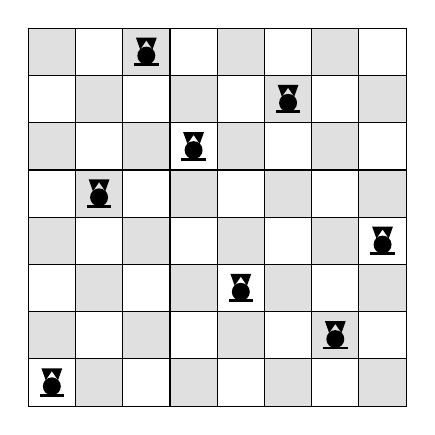
\begin{tikzpicture}[x = 6mm, y = 6mm]

% the board
\foreach \c in {0,...,7}
  \foreach \r in {0,...,7} {
    \pgfmathparse{Mod(\c+\r,2) == 0 ? "white" : "black!12"}
    \edef\shade{\pgfmathresult}
    \fill[\shade] (\c, \r) rectangle ++(1, 1);
  }
\draw[thin] (0, 0) rectangle (8, 8);
\foreach \i in {1,...,7} {
  \draw[thin] (\i, 0) -- (\i, 8);
  \draw[thin] (0, \i) -- (8, \i);
}

% one solution: the queens, drawn as a simple crowned disc
\foreach \c/\r in {0/0, 1/4, 2/7, 3/5, 4/2, 5/6, 6/1, 7/3} {
  \begin{scope}[shift={(\c+0.5, \r+0.5)}]
    \fill (0, -0.08) circle (0.19);
    \fill (-0.22, 0.30) -- (-0.13, 0.05) -- (0, 0.24) -- (0.13, 0.05)
          -- (0.22, 0.30) -- cycle;
    \fill (-0.26, -0.30) rectangle (0.26, -0.24);
  \end{scope}
}

\end{tikzpicture}
